This chapter offers an overview of the different implementation steps to develop the project.

\section{System Architecture Overview}

Follow low-level implementation detail of the different stages of the pipeline.\\

% \begin{figure}[h] 
% \centerline{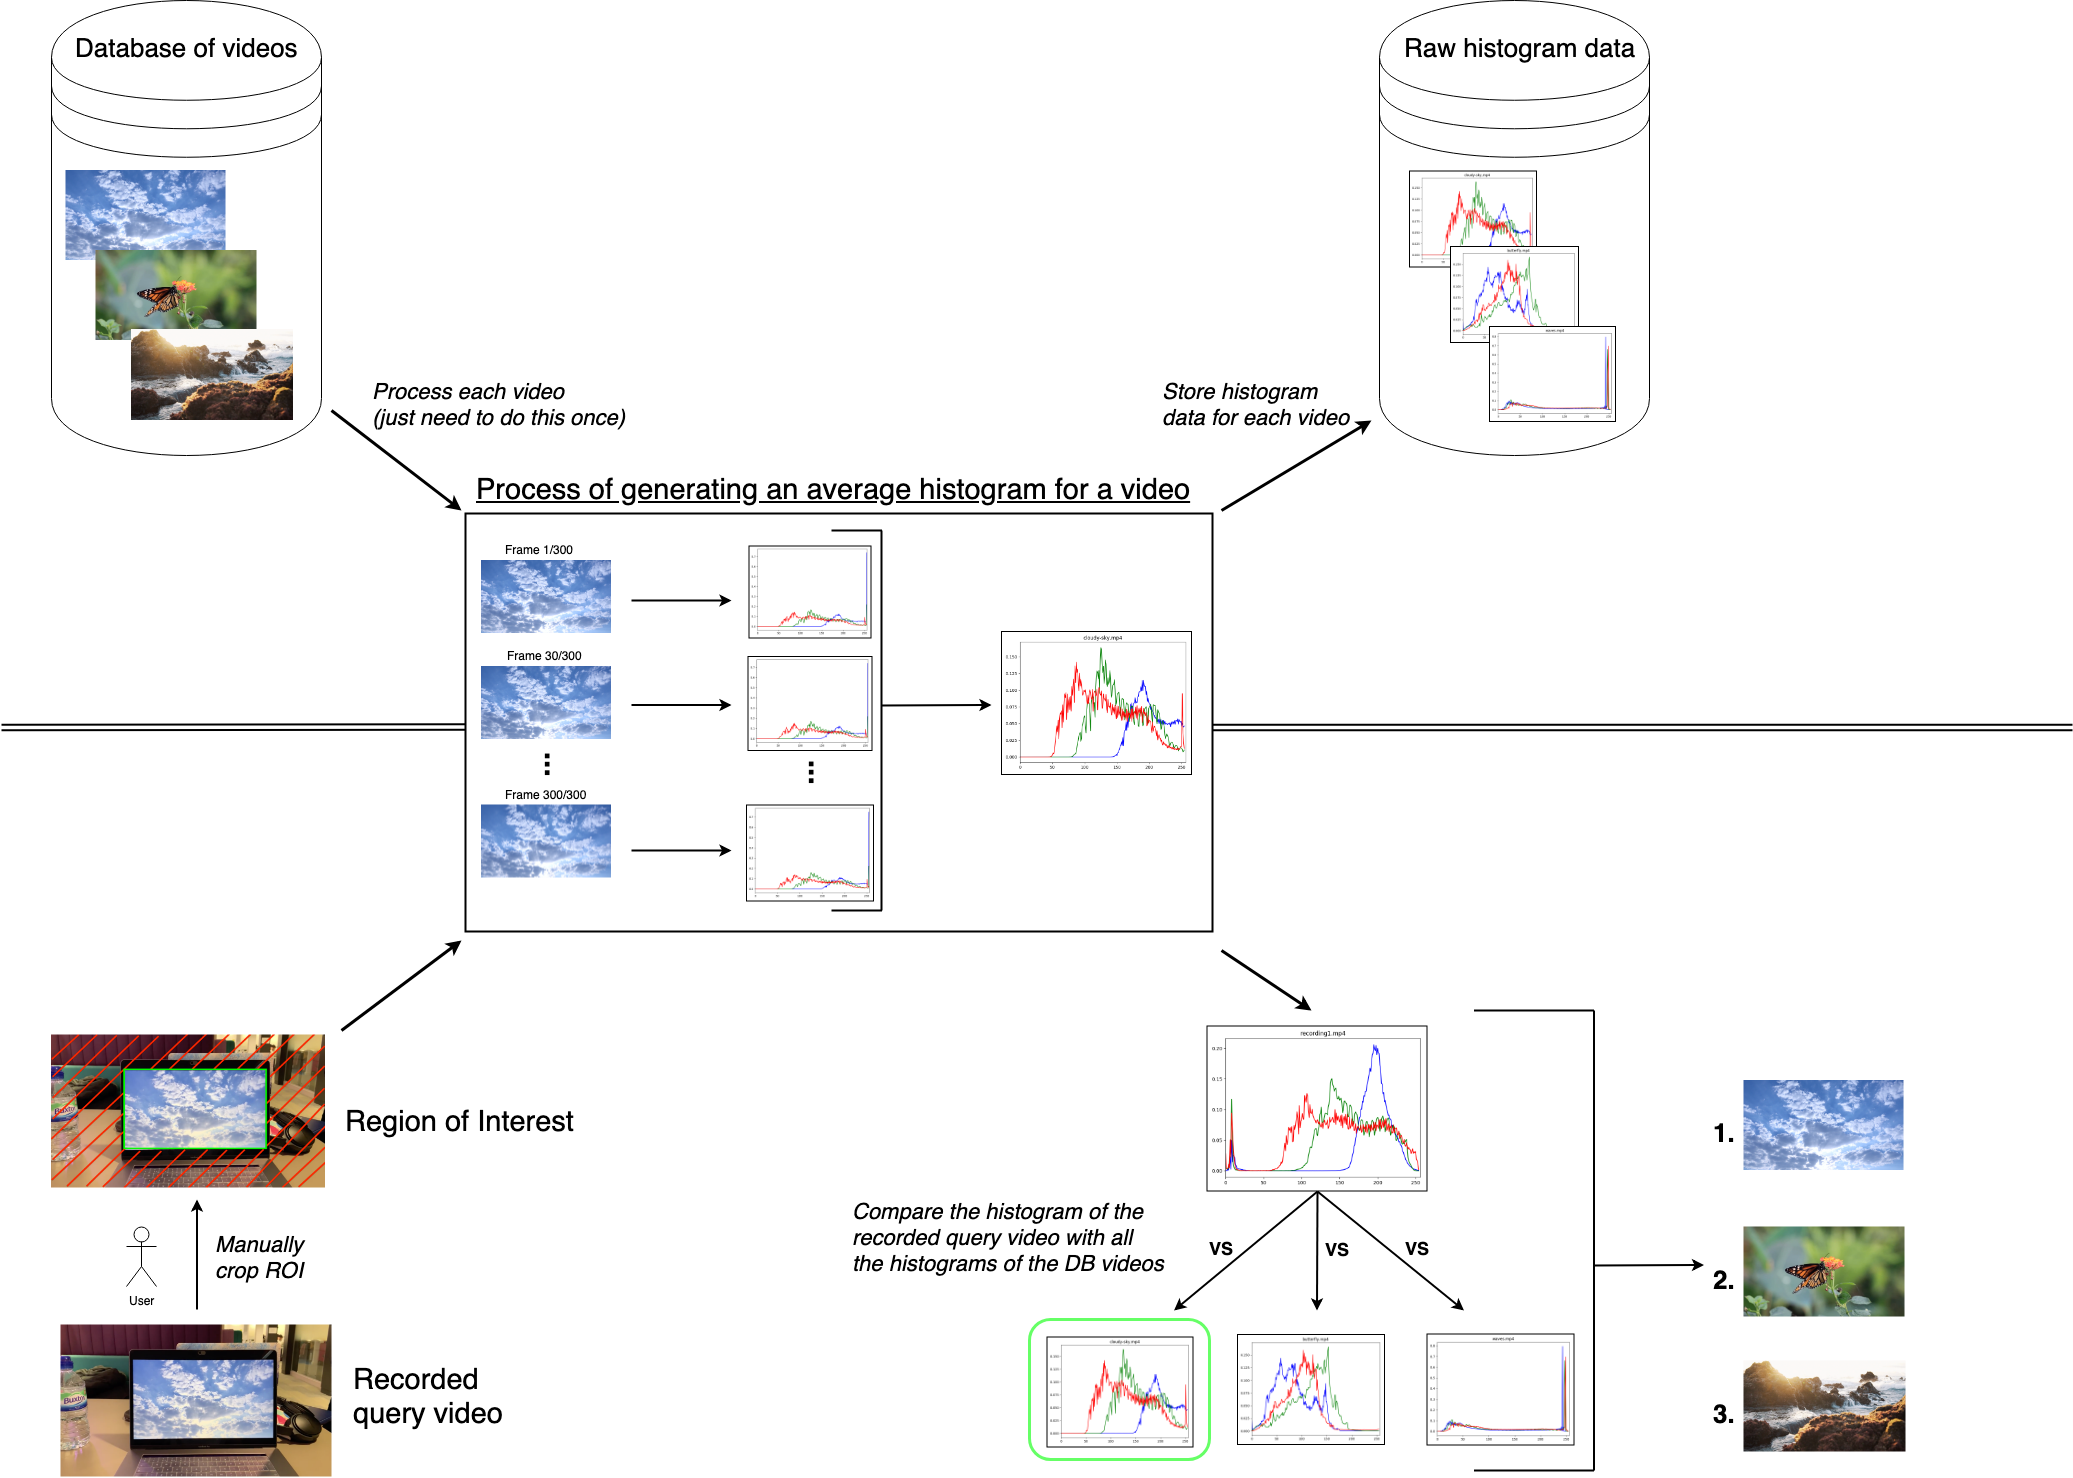
\includegraphics[width=\textwidth]{figures/implementation/CBVR-flowchart.png}}
% \caption{\label{fig:CBVR flowchart}Flowchart.}
% \end{figure}

%%%%%%%%%%%%%%%%%%%%%%%%%%%%%%%%%%%%%%%%%%%%%%%%%%%%%%%%%%%%%%%%%%%%
%%%%%%%%%%%%%%%%%%%%%%%%%%%%%%%%%%%%%%%%%%%%%%%%%%%%%%%%%%%%%%%%%%%%
%%%%%%%%%%%%%%%%%%%%%%%%%%%%%%%%%%%%%%%%%%%%%%%%%%%%%%%%%%%%%%%%%%%%

\section{Offline Colour-Based Feature Extraction}

This section details the different steps that go towards generating histograms and creating the compact signature used to represent each video. 

%%%%%%%%%%%%%%%%%%%%%%%%%%%%%%%%%%%%%%%%%%%%%%%%%%%%%%%%%%%%%%%%%%%%

\subsection{Histogram Generation}

As described in \ref{sec:color-based-features}, a histogram represents the distribution of the pixels in a single frame. Different types of histograms can be generated based on the colour model used. This section covers the generation of histograms in greyscale, RGB and HSV colour models, and how a single compact signature to represent videos can be created from these different histograms.\\

The array of stills that make a video can therefore be treated as images when creating the histograms.

%%%%%%%%%%%%%%%%%%%%%%%%%%

\subsubsection{Greyscale Histogram}

The first type of histogram that is generated is the greyscale histogram, also known as an intensity histogram. This type of histogram is used with frames that are converted to a black \& white colour space, and thus has a single channel rather than the three traditional RGB channels found in colour images. The conversion is done using OpenCV's \textit{cv2.cvtColor()} function along with the \textit{cv2.COLOR\_BGR2GRAY} attribute: 
\mint[fontsize=\footnotesize]{python}|grey_frame = cv2.cvtColor(frame, cv2.COLOR_BGR2GRAY)|

\begin{figure}[h] 
\centerline{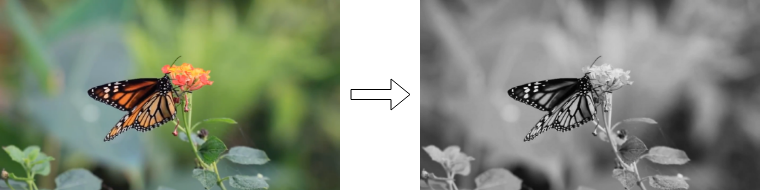
\includegraphics[width=\textwidth]{figures/implementation/rgb_to_greyscale.png}}
\caption{\label{fig:rgb_to_greyscale}Converting a frame from the RGB colour space to the greyscale.}
\end{figure}

Because the video frames are 8-bit images, the spectrum of the pixels values range between 256 possible values\footnote{$2^8=256$}. As a result, the histogram has 256 different bins ranging from 0 to 255 to represent all the potential values that each pixels can take. The histogram itself is calculated using Equation \ref{eq:grey-histogram}, where $g\in [0, 255]$ and $N_g$ represents the number of pixels that have an intensity equal to $g$.
\begin{equation}
\label{eq:grey-histogram}
    H(g)=N_g
\end{equation}

For example, $h(30)$ represents the number of pixels in the image with an intensity value of 30.\\

To implement the greyscale histogram generation in the system, OpenCV's \textit{calcHist()} method is used, with the result portrayed in Figure \ref{fig:implementation-greyscale_not_normalised}. The grey frame is passed to the function, along with the number of channels to use, which is a single one in this case ($[0]$), an empty mask $None$ since the histogram is being calculated for the full frame, the number of bins $[256]$, and the range of values $[0, 256]$:

\mint[fontsize=\footnotesize]{python}|histogram = cv2.calcHist([grey_frame], [0], None, [256], [0,256])|

\begin{figure}[h] 
\centerline{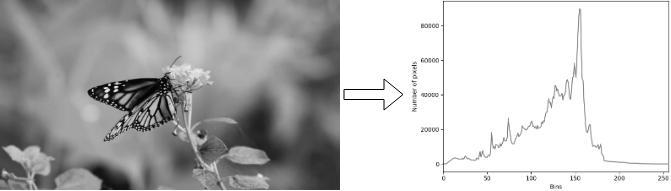
\includegraphics[width=\textwidth]{figures/implementation/greyscale_not_normalised.png}}
\caption{\label{fig:implementation-greyscale_not_normalised}The generated greyscale histogram (not normalised).}
\end{figure}

These greyscale histograms are generated for multiple frames of the video, but not all the frames as this would be highly inefficient (see Section \ref{sec:litsurvey-challenges-temporality}). Rather than generating a histogram for each frame, a selection of frames can be made in advance, which are then used for the histogram generation. Ideally, the frames extracted from the shot boundary detection algorithm are used. However, because the scope of the duration of the videos used is between 7 and 14 seconds and they are only made of a single shot, the shot boundary detection algorithm would only extract one frame. Therefore, for the purpose of testing, one frame is extracted every second to build up the selection of frames, using the \textit{\_get\_frames\_to\_process()} function from Appendix \ref{sec:code-listings-get-frames-to-process}. For example, with the butterfly video that contains 301 frames and has a frame rate of 30 frames per second, 11 frames are selected to generate greyscale histogram (frames \textit{[1, 31, 61, ..., 271, 301]}). Once the greyscale histograms are generated for each of these pre-selected frames, they are all stored away in a list, ready to be averaged into a single histogram that will be used as the compact signature to represent the entire video. 

%%%%%%%%%%%%%%%%%%%%%%%%%%

\subsubsection{RGB Histogram}

Next, RGB histograms are generated. As described in \ref{sec:color-based-features}, an RGB histogram represents the colour distribution of the pixels in a frame for three different channels: red, blue and green. The coloured frame is a combination of three colour channels, which can be split into threen different stills, as shown in Figure \ref{fig:implementation-rgb_image_channel_split}.

\begin{figure}[h] 
\centerline{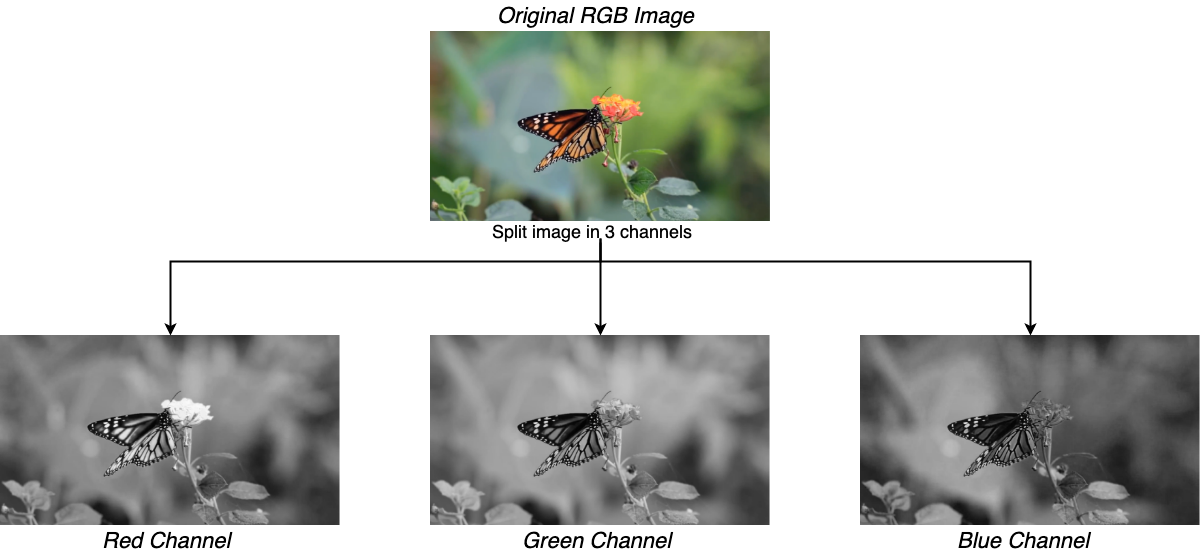
\includegraphics[width=\textwidth]{figures/implementation/rgb_image_channel_split.png}}
\caption{\label{fig:implementation-rgb_image_channel_split}The three colour channels that make up an coloured RGB image.}
\end{figure}

The RGB histogram is similar to the previous greyscale histograms, except that there are three separate 2D histograms, one for each channel (one in red, one in blue and one in green), where the brightness levels of each pixel are represented for each of those three colour channels. Each of the stills resulting from the split depicted in Figure \ref{fig:implementation-rgb_image_channel_split} will have their own histograms, which will form an RGB histogram when combined. Contrary to the greyscale histograms, frames do not need to be converted to a different colour space as they are directly imported into three channels. Similarly to the previous histogram, 256 bins are used for the RGB histograms, representing the potential values that each pixel can take for each colour channel. The RGB histogram is a combination of three 2D histograms, calculated using Equation \ref{eq:rgb-histogram}, where $g_i\in [0, 255]$ and $N_g^i$ represents the number of pixels that have an intensity equal to $g$ for the colour channel $i$. 

\begin{equation}
\label{eq:rgb-histogram}
    \sum_{i=0}^{2} H_i(g)=N_g[i]
\end{equation}

For example, $h_{i=2}(60)$ represents the number of pixels in the third channel of the image (blue channel) with an intensity value of 60.\\

To implement the RGB histogram, OpenCV's \textit{calcHist()} is once again used, with the results depicted in Figure \ref{fig:implementation-rgb_not_normalised}. In a similar fashion to the greyscale histogram, the frame is passed to the function along with the colour channel \textit{[i]}, which are all placed inside a for-loop to create a histogram for the three channels:

\mint[fontsize=\footnotesize]{python}|histogram = cv2.calcHist([frame], [i], None, [256], [0, 256])|

\begin{figure}[h] 
\centerline{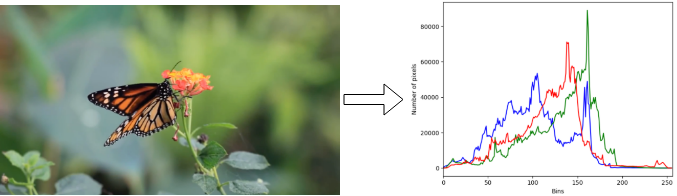
\includegraphics[width=\textwidth]{figures/implementation/rgb_not_normalised.png}}
\caption{\label{fig:implementation-rgb_not_normalised}The combination of the generated histograms for the three colour channels to construct the RGB histogram (not normalised).}
\end{figure}

Once all the RGB histograms have been generated for each of the pre-selected frames (one frame every second), they are all stored in a dictionary made up of three keys, one for each colour channel, which each link to a list where the histograms are stored away before being averaged into a single histogram used to create a second compact signature for the entire video. 

%%%%%%%%%%%%%%%%%%%%%%%%%%

\subsubsection{HSV Histogram Generation}

Finally, HSV histograms are the last type of histogram generated. HSV histograms make use of the HSV colour space, requiring the frames to be converted from the RGB colour space to HSV colour space. The conversion is done using OpenCV's \textit{cv2.cvtColor()} function along with the \textit{cv2.COLOR\_BGR2HSV} attribute:

\mint[fontsize=\footnotesize]{python}|hsv_frame = cv2.cvtColor(frame, cv2.COLOR_BGR2HSV)|

\begin{figure}[h] 
\centerline{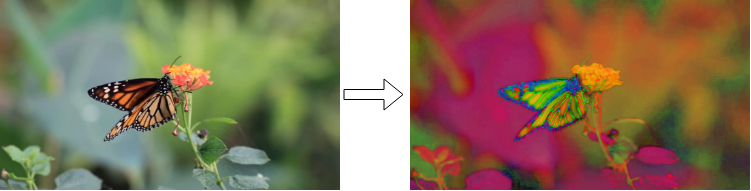
\includegraphics[width=\textwidth]{figures/implementation/rgb_to_hsv.png}}
\caption{\label{fig:greycale_histogram_generation}Converting a frame from the RGB colour space to the HSV colour space.}
\end{figure}

This type of histogram is more complex to generate as it is not a 2D histogram like the previous greyscale and RGB histograms, but a 3D histogram. Because they are represented in 3D rather than 2D due to the particularities of the HSV colour space, less bins can be used to plot the data as pixels fall into bins when they are within in conjunction in the range of the three channels. Therefore, to avoid creating a histogram that is neither too coarse and neither too dense, 8 bins are used for the hue channel, 12 bins are used for the saturation channel, and 3 bins are used for the value channel. This results in a histogram of 288 values\footnote{$8*12*3=288$}, which is approximately the same length as the 256 values that were previously used for the greyscale histograms and $256*3$ values for the RGB histograms. The histogram is constructed using Equation \ref{eq:hsv-histogram}, where $N(h,s,v)$ represents the number of pixels that fall within the range of the bin with values $h$ \underline{AND} $s$ \underline{AND} $v$.\\
\begin{equation}
\label{eq:hsv-histogram}
    H(h,s,v)=N(h,s,v)
\end{equation}

For example, a pixel with values $H(h=31, s=245, v=200)$ will fall into the bin with a hue value between 22.5 and 45 (bin \#2/8) \underline{AND} saturation value between 234.6 and 256 (bin \#12/12) \underline{AND} value intensity between 170.7 and 256 (bin \#3/3). The number of pixels in this bin will be $N(1,11,2)$ (0-based indexes).\\

Implementing an HSV histogram is again achieved through the use of OpenCV's \textit{calcHist()} function, with the result shown in Figure \ref{fig:implementation-hsv_not_normalised}. Similar arguments are passed such as the frame and an empty mask, but the arguments controlling the size of the histogram are different. \textit{[0, 1, 2]} indicates that the histogram has three channels, \textit{(8, 12, 3)} specifies the number of bins, and \textit{[0, 180, 0, 256, 0, 256]} markes the ranges of these bins:

\mint[fontsize=\footnotesize,breaklines]{python}|histogram = cv2.calcHist([hsv_frame], [0, 1, 2], None, (8, 12, 3), [0, 180, 0, 256, 0, 256])|

\begin{figure}[h] 
\centerline{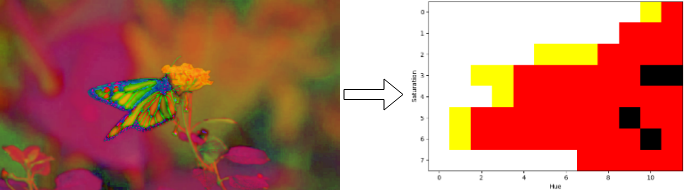
\includegraphics[width=\textwidth]{figures/implementation/hsv_not_normalised.png}}
\caption{\label{fig:implementation-hsv_not_normalised}The generated 3D HSV histogram (not normalised).}
\end{figure}

To conclude, the same steps are followed for HSV histograms. Once all the HSV histograms have been generated for each pre-selected frame, they are all stored in a list until they are averaged into a compact histogram.

\begin{listing}[h]
\inputminted
[
baselinestretch=0.9,
bgcolor=LightGray,
fontsize=\footnotesize,
linenos,
breaklines,
]
{python}{code-listings/generate_single_histogram.py}
\caption{Function generating histograms for the pre-selected frames and adding them to lists before averaging them to create a video's compact signature.}
\label{listing:generate_single_histogram}
\end{listing}

%%%%%%%%%%%%%%%%%%%%%%%%%%%%%%%%%%%%%%%%%%%%%%%%%%%%%%%%%%%%%%%%%%%%

\subsection{Compact Video Signature}

averaging histogram
normalising
writing to human-readable txt file
1 frame every 30 frames retrieved

% \begin{figure}[h] 
% \centerline{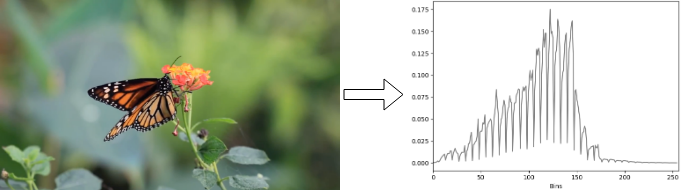
\includegraphics[width=\textwidth]{figures/implementation/greycale_histogram_generation.png}}
% \caption{\label{fig:greycale_histogram_generation}Example of the generated greyscale histogram.}
% \end{figure}

% \begin{figure}[h] 
% \centerline{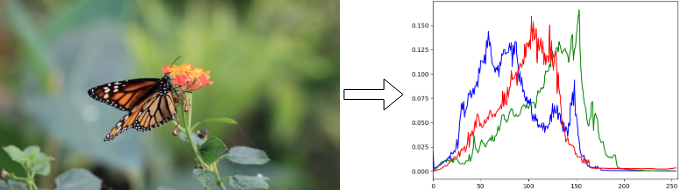
\includegraphics[width=\textwidth]{figures/implementation/rgb_histogram_generation.png}}
% \caption{\label{fig:implementation-rgb_histogram_generation}Example of the three generated RGB histogram channels.}
% \end{figure}

% \begin{figure}[h] 
% \centerline{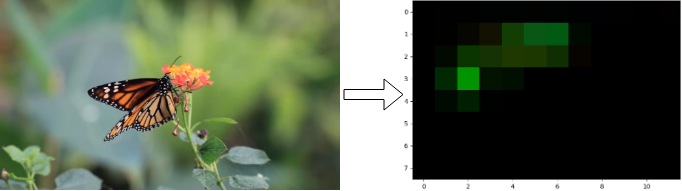
\includegraphics[width=\textwidth]{figures/implementation/hsv_histogram_generation.png}}
% \caption{\label{fig:hsv_histogram_generation}Example of the generated HSV histogram.}
% \end{figure}

%%%%%%%%%%%%%%%%%%%%%%%%%%%%%%%%%%%%%%%%%%%%%%%%%

%%%%%%%%%%%%%%%%%%%%%%%%%%%%%%%%%%%%%%%%%%%%%%%%%%%%%%%%%%%%%%%%%%%%
%%%%%%%%%%%%%%%%%%%%%%%%%%%%%%%%%%%%%%%%%%%%%%%%%%%%%%%%%%%%%%%%%%%%
%%%%%%%%%%%%%%%%%%%%%%%%%%%%%%%%%%%%%%%%%%%%%%%%%%%%%%%%%%%%%%%%%%%%

\section{Online Retrieval}

query video, identical features extracted

\subsection{Query Video Pre-processing}

\subsubsection{Video Stabilisation}

video stabilised

\subsubsection{Region of Interest Selection}

roi selection

\subsection{Similarity Measurements}

distance measurements to find nearest neighbour between query histograms and each database video histogram:

\begin{itemize}
    \item correlation
    \item intersection
    \item chi-square
    \item alternative chi-square
    \item bhattacharyya
    \item kullback leibler divergence
    \item wassertein distance (Earth's Mover Distance)
    \item energy distance
\end{itemize}

combining results from all 3 methods with weight between different histogram methods to give more importance to HSV, GRB and less importance to grey scale: 1-5-10

%%%%%%%%%%%%%%%%%%%%%%%%%%%%%%%%%%%%%%%%%%%%%%%%%%%%%%%%%%%%%%%%%%%%
%%%%%%%%%%%%%%%%%%%%%%%%%%%%%%%%%%%%%%%%%%%%%%%%%%%%%%%%%%%%%%%%%%%%
%%%%%%%%%%%%%%%%%%%%%%%%%%%%%%%%%%%%%%%%%%%%%%%%%%%%%%%%%%%%%%%%%%%%

\section{Database Pre-Processing}

\begin{itemize}
    \item shot boundary detection for long videos, allowing the entire movie to be represented with a few thousand frames
    \item current: one frame every second for short videos
\end{itemize}

%%%%%%%%%%%%%%%%%%%%%%%%%%%%%%%%%%%%%%%%%%%%%%%%%%%%%%%%%%%%%%%%%%%%
%%%%%%%%%%%%%%%%%%%%%%%%%%%%%%%%%%%%%%%%%%%%%%%%%%%%%%%%%%%%%%%%%%%%
%%%%%%%%%%%%%%%%%%%%%%%%%%%%%%%%%%%%%%%%%%%%%%%%%%%%%%%%%%%%%%%%%%%%

\section{Output-Related}

\begin{itemize}
    \item opencv box drawing to select Region of Interest
    \item matplot lib histogram plotting (with an option to show each generated histogram or to hide them)
    \item tables to show scores for each type of histogram and each distance
    \item exporting results to CSV for further analysis
    \item spinners to show calculations are being done when training the system or stabilising videos 
    \item argument parsing
    \item final output to clearly show if result if right/wrong, including a frame of the original query video, a frame of the match found, along with the runtime and tha accuracy
\end{itemize}

%%%%%%%%%%%%%%%%%%%%%%%%%%%%%%%%%%%%%%%%%%%%%%%%%%%%%%%%%%%%%%%%%%%%
%%%%%%%%%%%%%%%%%%%%%%%%%%%%%%%%%%%%%%%%%%%%%%%%%%%%%%%%%%%%%%%%%%%%
%%%%%%%%%%%%%%%%%%%%%%%%%%%%%%%%%%%%%%%%%%%%%%%%%%%%%%%%%%%%%%%%%%%%

\section{Testing}

\begin{itemize}
    \item Unit Testing
        \begin{itemize}
            \item grey scale / RGB / HSV histogram generation
            \item histogram saving to file
            \item histogram normalisation
            \item ROI selection
            \item individual histogram matching, test each metric
        \end{itemize}
    \item Integration Testing
        \begin{itemize}
            \item test the entire pipeline (with a few videos as the database, make sure the correct match is found)
        \end{itemize}
    \item Include some code snippets
    \item Include test suite results
\end{itemize}